\section{Comparison data simulation}
Now that  we have a  good simulation of  each step of  the electronics
chain, we  want to test  the simulation with  the data. One way  to do
that is  by looking at  the fluctuations of  the radio signal  that we
measure in the recorded events. So we will carry out a full simulation
and compare the distribution of the  radio signal in ADC units. 
\subsection{data}
To measure the RMS of the  detectors installed in the field, we select
events with EASIER stations hit  and just histogram the radio waveform
in ADC (after  removing the baseline). We have  picked arbitrarely the
month  of  April 2015  (it  is  the period  when  all  the arrays  are
present).  We  show as an example  3 waveforms, one for  each array of
the C-band  in the  figure~\ref{fig:datatrace} (left) and  the average
RMS  is shown  for all  the stations  during the  chosen month  in the
figure~\ref{fig:datatrace} (right). Most of the EASIER61 detector have
their RMS around  50 ADCs and some  of them are a little  off and some
close to  zero.  For the  EASIER7 array the  RMS is lower  because the
capacitor  is  present after  the  power  detector.   Finally all  the
GIGADUCK detectors (except one) have their RMS between 47 and 50 ADCs.

\begin{figure}[!ht]
  \centering
  \hspace*{-3ex}
  \subfigure{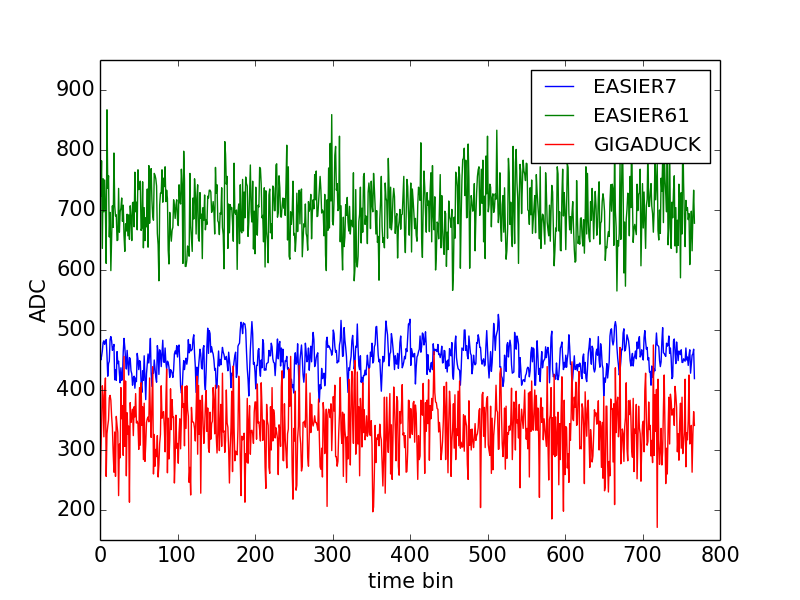
\includegraphics[width=0.49\linewidth]{datatrace.png}}
  \subfigure{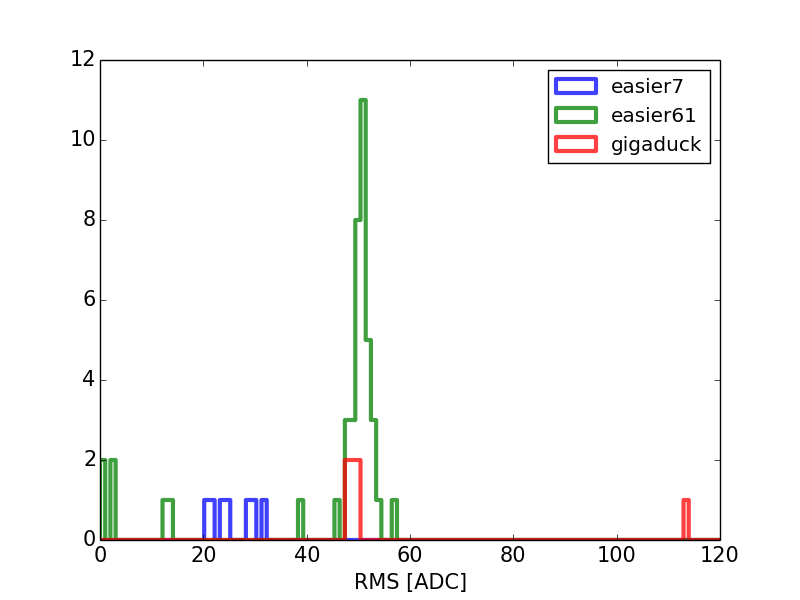
\includegraphics[width=0.49\linewidth]{datarmsdist.png}}
  \caption{example of trace from each detector in the C-band. right: distribution of the average RMS of all detectors}
  \label{fig:datatrace}
\end{figure}

\begin{figure}[!ht]
  \centering
  \hspace*{-3ex}
  \subfigure{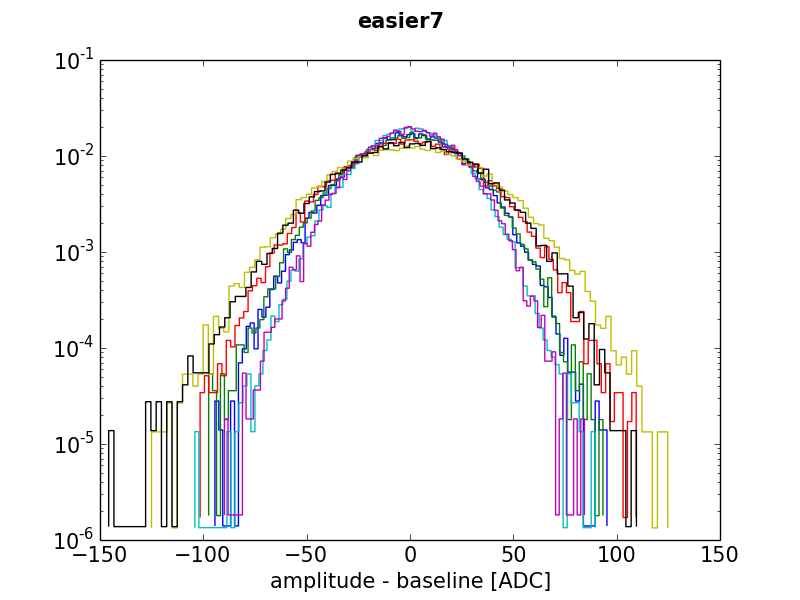
\includegraphics[width=0.32\linewidth]{disteasier7.png}}
  \subfigure{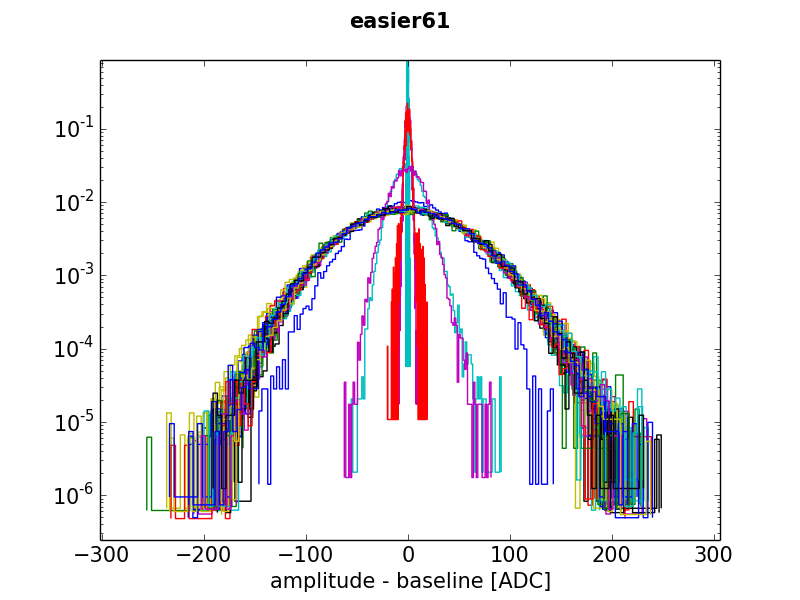
\includegraphics[width=0.32\linewidth]{disteasier47.png}}
  \subfigure{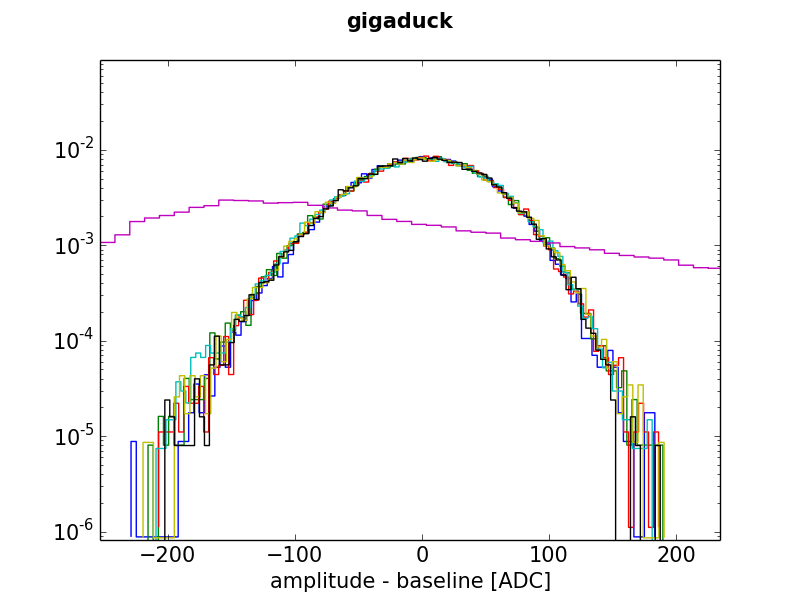
\includegraphics[width=0.32\linewidth]{distgigaduck.png}}
  \caption{example of  trace from each detector in  the C-band. right:
    distribution of the average RMS of all detectors.}
  \label{fig:datatrace}
\end{figure}

\subsubsection{simulation}
Now    we   can    produce    HF   waveforms    from   the    measured
spectra~\ref{sec:rf},   then  make   the  waveform   go   through  the
electronics  simulation we  described  in section~\ref{sec:elec}.   We
show  here  the  results  for  the three  methods  of  power  detector
simulation.    Figure~\ref{fig:m1_distdata},   ~\ref{fig:m2_distdata},
~\ref{fig:m3_distdata} show the measured and simulated distribution of
amplitude in ADC counts, and figure~\ref{fig:compmeanrms} compares the
average RMS (we removed the bad stations).

\begin{figure}[!ht]
  \centering
  \hspace*{-3ex}
  \subfigure{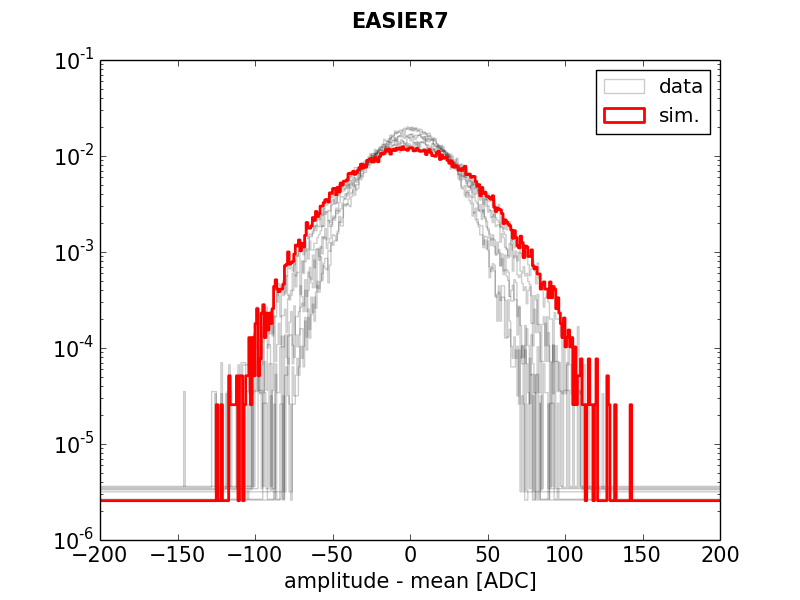
\includegraphics[width=0.32\linewidth]{m1_distdatasimEA7.png}}
  \subfigure{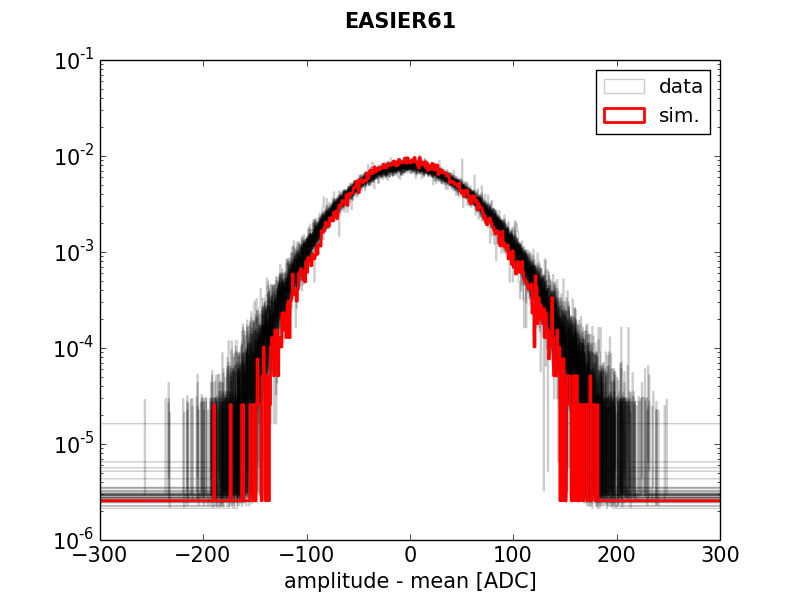
\includegraphics[width=0.32\linewidth]{m1_distdatasimEA61.png}}
  \subfigure{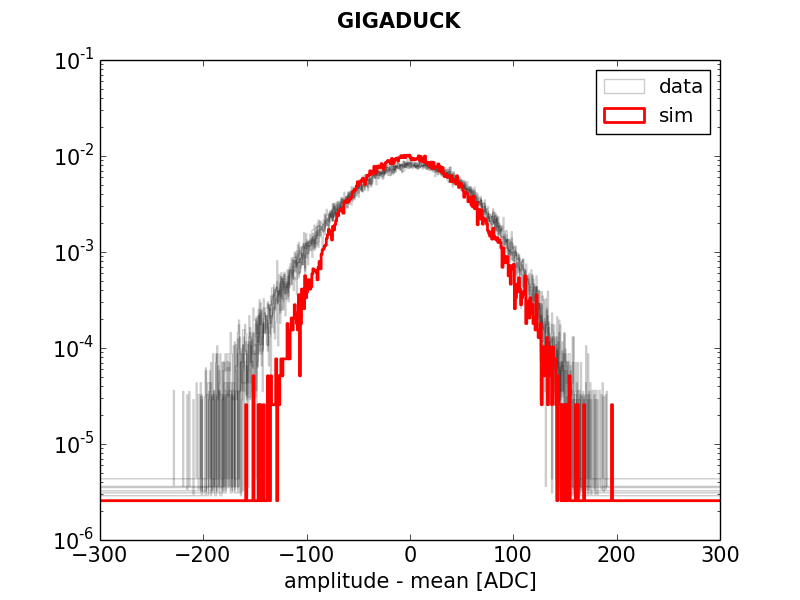
\includegraphics[width=0.32\linewidth]{m1_distdatasimGD.png}}
  \caption{method 1: comparison of the measured distribution of amplitude and the simulated one.}
  \label{fig:m1_distdata}
\end{figure}

\begin{figure}[!ht]
  \centering
  \hspace*{-3ex}
  \subfigure{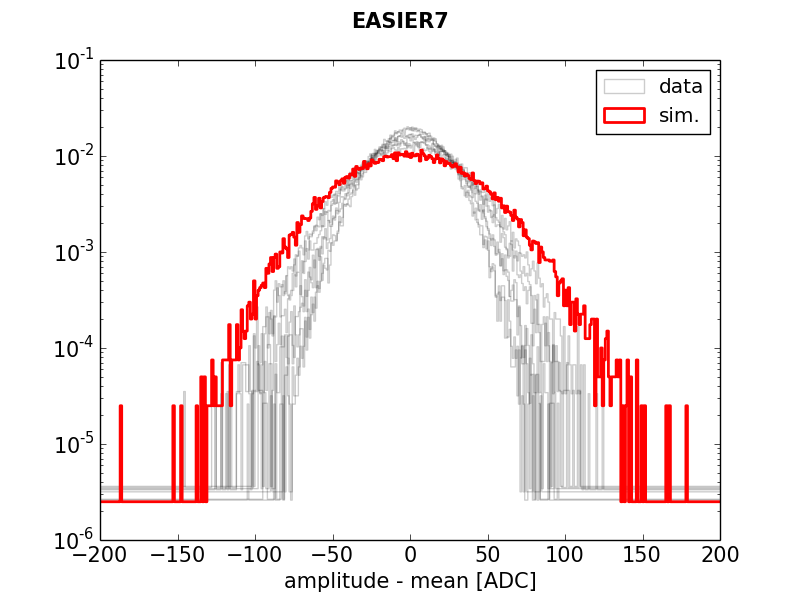
\includegraphics[width=0.32\linewidth]{m2_distdatasimEA7.png}}
  \subfigure{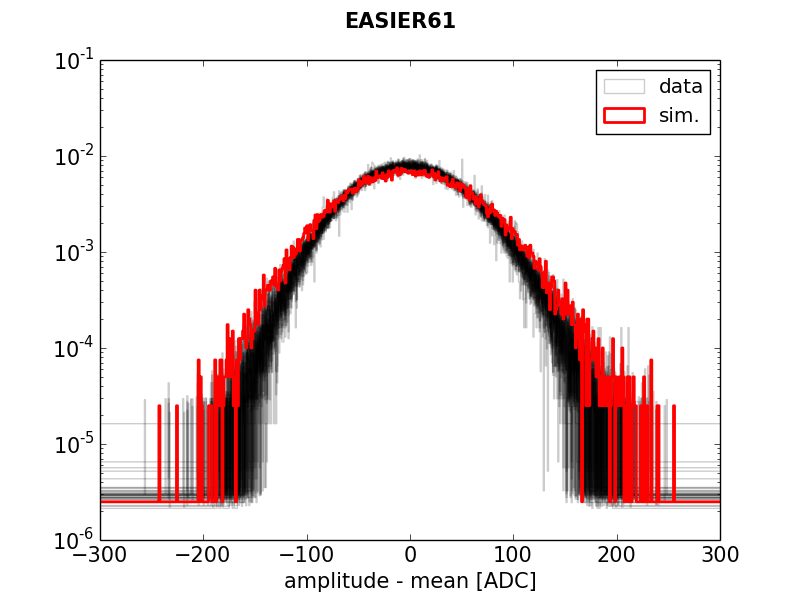
\includegraphics[width=0.32\linewidth]{m2_distdatasimEA61.png}}
  \subfigure{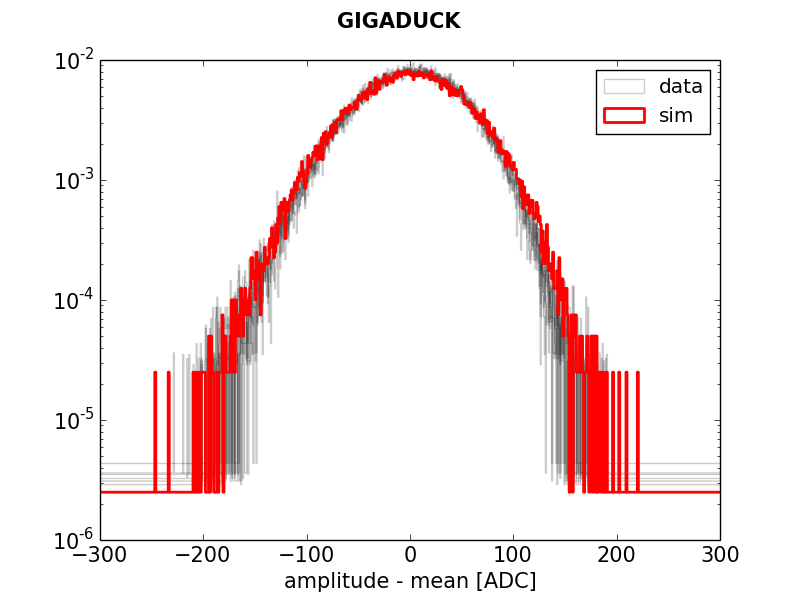
\includegraphics[width=0.32\linewidth]{m2_distdatasimGD.png}}
  \caption{method 2: comparison of the measured distribution of amplitude and the simulated one.}
  \label{fig:m2_distdata}
\end{figure}

\begin{figure}[!ht]
  \centering
  \hspace*{-3ex}
  \subfigure{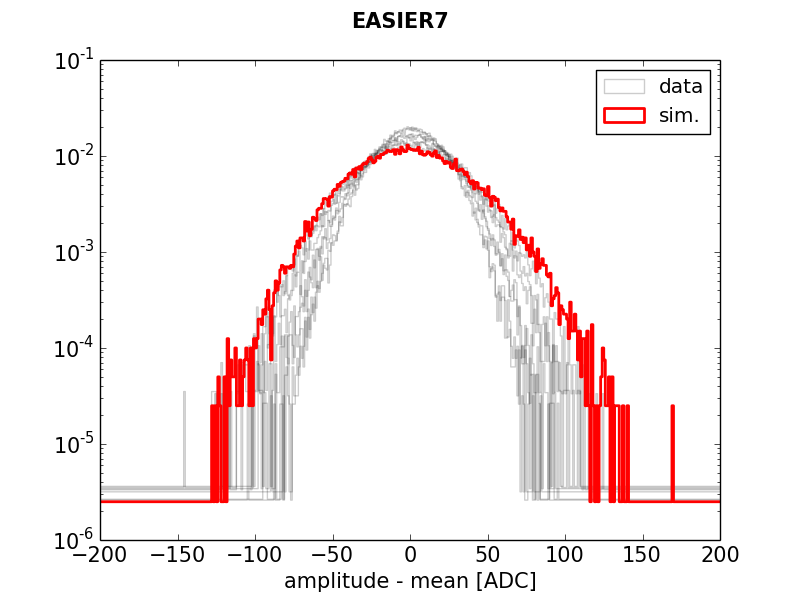
\includegraphics[width=0.32\linewidth]{m3_distdatasimEA7.png}}
  \subfigure{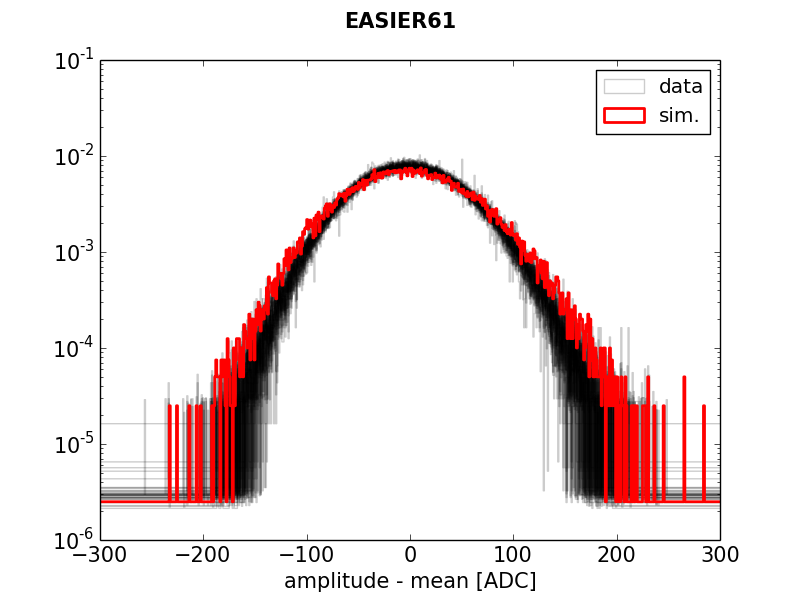
\includegraphics[width=0.32\linewidth]{m3_distdatasimEA61.png}}
  \subfigure{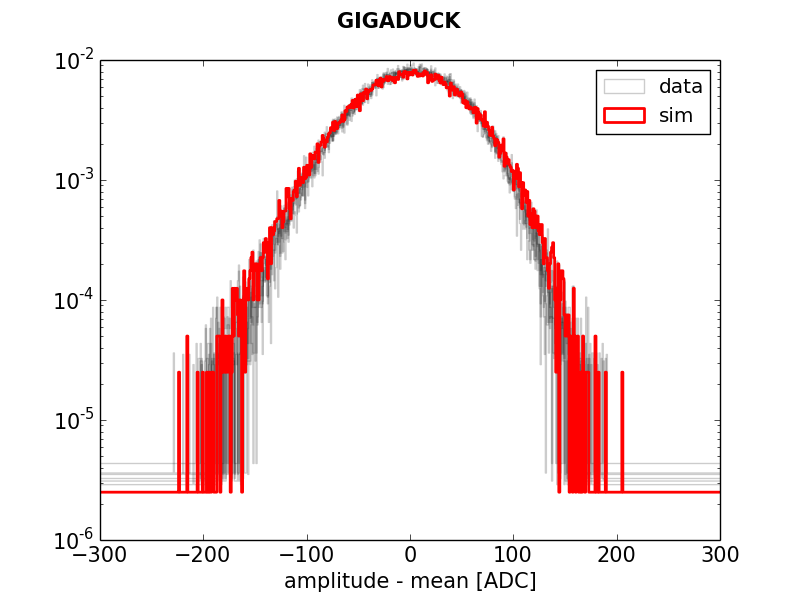
\includegraphics[width=0.32\linewidth]{m3_distdatasimGD.png}}
  \caption{method 3: comparison of the measured distribution of amplitude and the simulated one.}
  \label{fig:m3_distdata}
\end{figure}

\begin{figure}[!ht]
  \centering
  \hspace*{-3ex}
  \subfigure{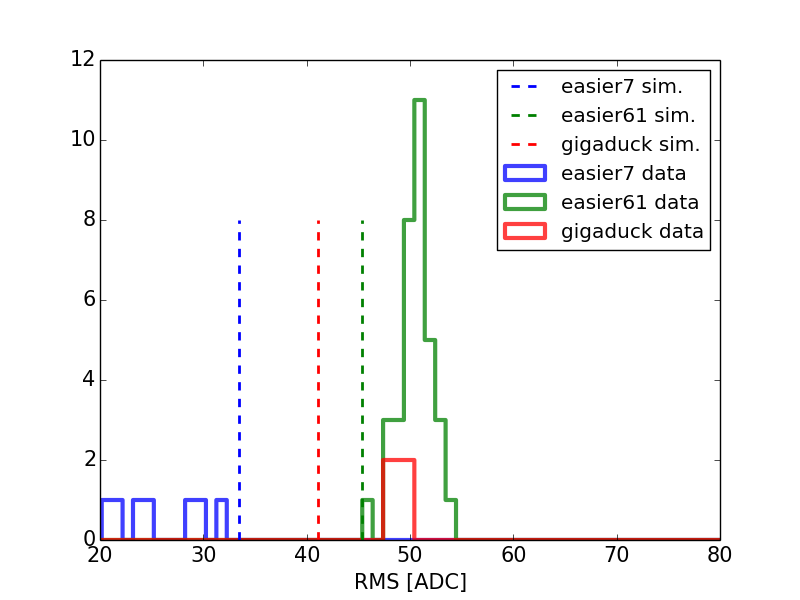
\includegraphics[width=0.33\linewidth]{datasimrmsdist.png}}
  \subfigure{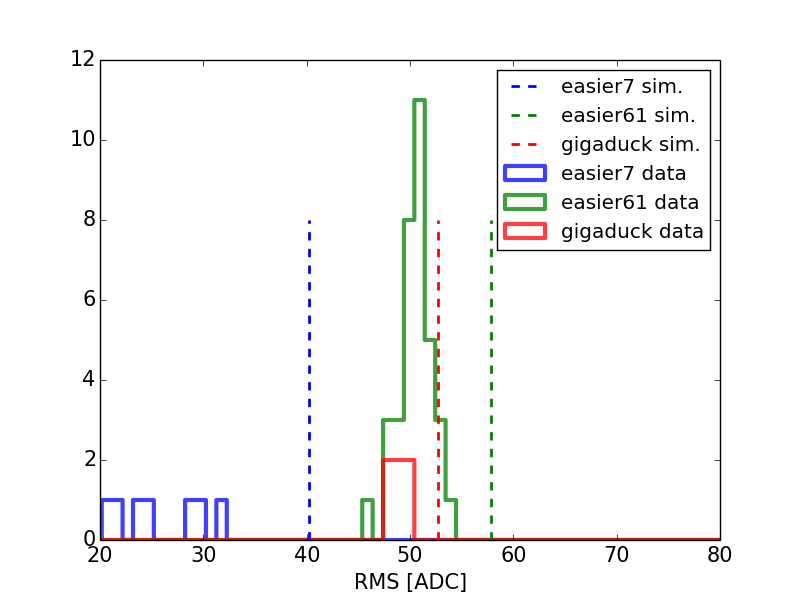
\includegraphics[width=0.33\linewidth]{m2_datasimrmsdist.png}}
  \subfigure{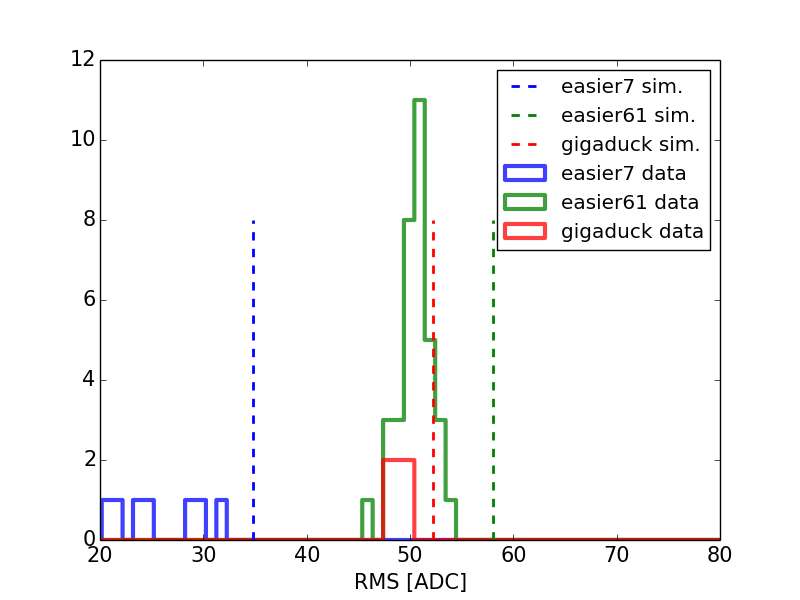
\includegraphics[width=0.33\linewidth]{m3_datasimrmsdist.png}}
  \caption{comparison of the measured distribution of amplitude and the simulated one.}
  \label{fig:datatrace}
\end{figure}

At the  end, the three method  give very close results,  the first one
yields a larger RMS for the  capacitor case, but a smaller one for the
non capacitor case.  The two  other give consistantly a larger RMS for
the three  detector configurations. Note that the  difference is quite
small, only  a few ADC  counts.  (50  ADC is 1dB  and we have  at most
differences of around 15 ADC i.e. less than 10$\rm \%$)
%% At the  end, none of  the method finds  the correct value. But  we get
%% numbers very close to the data. 



%% At the end  the average value of the RMS are  smaller for EASIER61 and
%% GIGADUCK and larger for EASIER7. I  think that the reason might be the
%% parameters found in  section 1. When I fit the  time constant I obtain
%% at  the  same time  the  characteristic of  the  power  detector (V  =
%% f(power)). When we look  at the value a and b obtain  for the two case
%% we see that they are different and the final fluctuation are sensitive
%% to  the parameter  a  (the slope).   Especially  we see  that for  the
%% capacitor case the  slope is larger than the  no capacitor case, which
%% goes in the  same trend as the  discrepancy in the RMS (I  mean if the
%% value of a was taken as the  mean of the two value we would reduce the
%% discrepancies of both cases.) Another possibility is that the response
%% is a  little different for the noise  part and the signal  part. In my
%% thesis I had found a difference  in the fit results for the noise part
%% and the signal part. 
 


